\documentclass[interim_report.tex]{subfiles}

\begin{document}

\section{Introduction}
\subsection{Motivation}
As modern computing techniques advance, people are trying to find more generic solutions to problems which have been solved by native applications in the past. A main area of focus has been network middleboxes (Figure~\ref{fig:middlebox}), which are developed to manipulate network packets. Common examples of middleboxes are firewalls, network address translators (NATs) and load balancers, all of which inspect or transform network packets in the middle of a connection between a public and private network. In recent years, people have been developing a number of programmable middleboxes which allow these generic solutions to be used on a wide scale basis.

\begin{figure}[H]
	\centering
	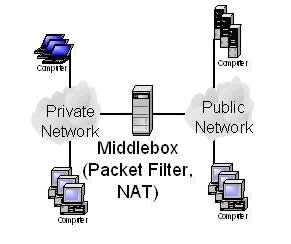
\includegraphics[scale=0.75]{img/middleboxes.jpg}
	\caption{Middlebox Example \cite{middlebox}}
	\label{fig:middlebox}
\end{figure}

\noindent As middleboxes are mainly used for networking purposes, they are required to process network packets at line rate (i.e. at speeds which allow packets to be processed as they are received). This requires the application to retrieve the packet from the network line, inspect and transform the packet in the desired way and then insert the packet back onto the network line, all within a time period sufficient enough to not cause a backlog. High performance implementations of such applications are available, but are written in native languages, predominately in C/C++. However, more and more high performance computing projects are been developed in Java and have succeeded in performing at similar speeds to C/C++ applications. \\
\newline
The main challenge is actually getting the I/O system for the Java application to run at line rate speeds, due to challenges with how the JVM (Java Virtual Machine) interacts with memory and the computer's kernel. Once this challenge has been overcome, there are no reasons why programmable middleboxes written in none native languages such as Java can't exist within networking systems.

\subsection{Objectives}
The main objective for this project is to research, develop and test a new application which is implemented in a non-native language such as Java, but can process packets at a high performance level. This also requires that the application can perform I/O operations at line rate in order to pass on data packets without reducing the line rate. The aim is to match current native applications which are generally written in C/C++. \\
\newline
With the main objective stated above, I set out a few initial, smaller objectives in order to divide the project into more manageable objectives:
\begin{itemize}
	\item Understand similar applications and API's written in C/C++ which process at line speeds and how the implementations can be exploited for Java applications
	\item Conduct research into Java techniques which can be used in order to increase I/O operations
	\item Implement basic middlebox applications in Java such as a firewall and a NAT
	\item Compare Java implementations to those which are pure Java and pure C/C++
\end{itemize}

\subsection{Solution Idea}
The idea is to implement a new library in Java using a few techniques in order to speed up network access. Firstly, no networking will be done via the JVM and the operating system kernel. Instead, the Java application will bypass the kernel altogether using a combination of direct memory access and high speed I/O operations via a C library which we interact with the application via the Java Native Interface (JNI). \\
\newline
This eliminates the need for the JVM to interact with the kernel via system calls in order to do the network access, which can be relatively slow compared to direct network access achievable from native applications.

\end{document}